\documentclass[a4paper, 11pt]{article}
\usepackage{comment} % enables the use of multi-line comments (\ifx \fi)  
\usepackage{fullpage} % changes the margin
\usepackage{graphicx}
\begin{document}
%Header-Make sure you update this information!!!!
\noindent
\large\textbf{Homework Assignment X} \hfill \textbf{Anirudh Ganesh} \\
\normalsize Computer Vision for HCI \hfill CSE5524 (Au `18) \\
Prof. Jim Davis \hfill Score: \_\_\_/12 \\
TA: Sayan Mandal \hfill Due Date: 11/13/18

\section*{PART A: Back Propagation}

\begin{figure}[h]
\centering
  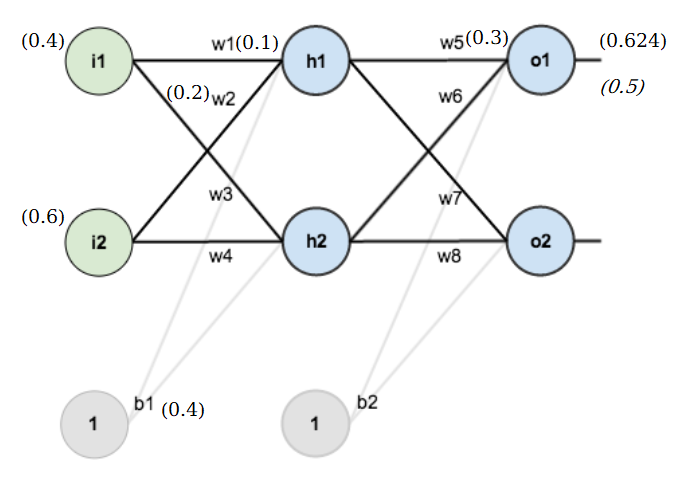
\includegraphics[scale=0.4]{backprop.png}
  \caption{The given network.}
\end{figure}


Goal is to determine the new weight parameter $w_5$ after one cycle of Gradient Descent using the single example given to us.

$$\frac{\partial E_{total}}{\partial w_5} = \frac{\partial E_{total}}{\partial out_{01}} * \frac{\partial out_{01}}{\partial net_{01}} * \frac{\partial net_{01}}{\partial w_5}$$

\subsection*{Calculating gradient of error}

The error function is given as,

$$ E_{total} = \frac{1}{2}(target_{01} - out_{01})^2 + \frac{1}{2}(target_{02} - out_{02})^2$$

\noindent Thus, the gradient of error is given as,

$$ \frac{\partial E_{total}}{\partial out_{01}} =  -(target_{01} - out_{01}) = -(0.5 - 0.624) = 0.124$$

\subsection*{Calculating $\Delta out_{01}$}

Output layer is given by,

$$ out_{01} = \frac{1}{1+e^{-net_{01}}}$$

\noindent Thus the $\Delta out_{01}$ is given by,

$$ \frac{\partial out_{01}}{\partial net_{01}} = out_{01} * (1 - out_{01}) = (0.624) * (1 - 0.624) = 0.235$$

\subsection*{Calculating $\Delta net_{01}$}

Net activation for the layer is given by,

$$ net_{01} = w_5 * out_{h1} + w_6 * out_{h2} + b_2$$

\noindent Thus the $\Delta net_{01}$ can be computed as,

$$ \frac{\partial net_{01}}{\partial w_5} = out_{h1} $$

\noindent In order to compute $out_{h1}$, we need $net_{h1}$,

$$ net_{h1} = i_1*w_1 + i_2 * w_2 + b_1 = (0.4*0.1) + (0.6*0.2) + 0.4 = 0.04 + 0.12 + 0.4 = 0.56$$

\noindent From this we compute $out_{h1}$ as,

$$ out_{h1} = \frac{1}{1+e^{-net_{h1}}} = \frac{1}{1+e^{-0.56}} = 0.636$$

\noindent Coming back to our $\Delta net_{01}$,

$$ \frac{\partial net_{01}}{\partial w_5} = out_{h1} = 0.636$$

\subsection*{Compute the step for gradient descent}

$$\frac{\partial E_{total}}{\partial w_5} = \frac{\partial E_{total}}{\partial out_{01}} * \frac{\partial out_{01}}{\partial net_{01}} * \frac{\partial net_{01}}{\partial w_5} = 0.124 * 0.235 * 0.636 = 0.019$$

\subsection*{Update the weight, $\alpha = 0.3$}

$$w_5 = w_5 - \alpha \frac{\partial E_{total}}{\partial w_5} = 0.3 - 0.3 * 0.019 = 0.294$$

\section*{PART B: Convolutional Neural Networks}

So we start off straight off the shelf with a pretty good baseline of $96.76\%$. In-order to improve the accuracy from the baseline, I tried a couple of things. 

First of all was experimenting the the different filter size of the first convolutional layer. After some tweaking a filter size of 3, and a filter number of 32 was found to be the optimal. This change bumped up the models performance to $96.96\%$.

The next major change was to add a fully connected layer of 128 nodes before the classifying layer. To mitigate the slowdown in training, batch size was bumped up to 512. These changes give us our best performance of $97.98\%$.

Now, in-order to further increase performance, it was clear that I had to incorporate multiple convolutional layers. But try as I might, in different orders and combinations, the code given utilized the convolutional layer in a format that was unfamiliar to me. So I re-created the similar model with a similar performance in Keras and Python using a Tensorflow backend with a new baseline of $95.48\%$. After this, I was able to add two sets of 64,3 2d convolutional layer, followed by a maxpool of 2x2, followed by two convolution of 128, 3 followed by another maxpool of 2x2. Finally a dense network of 256 and a softmax (all with ReLU activation by default). This gives the best performance of $99.73\%$. I then converted these weights from Keras's h5 format to mat format. Though I don't know how grader is going to utilize this hence this model is submitted separately.

\end{document}
